\documentclass[12pt]{article}
\frenchspacing
\usepackage[utf8x]{inputenc}
\usepackage[T2A]{fontenc}
\usepackage{amsmath}
\usepackage{amsfonts}
\usepackage{amssymb}
\usepackage[russian]{babel}
\usepackage{graphicx}
\usepackage{hyperref}
\usepackage{multirow}
\usepackage[left=2cm,right=2cm,top=2cm,bottom=2cm,bindingoffset=0cm]{geometry}
\author{Рашковецкий М.М., группа 526т}
\date{\today}
\title{Лабораторная работа 2.3.1\\Получение и измерение вакуума}

\newcommand{\degC}{^\circ \text{C}}
\newcommand{\fref}[1]{рис. \ref{#1}}

\begin{document}
	\maketitle
	
	{\parindent=1cm \hangindent=1cm \parskip=0.5cm
	{\bfseries Цель работы:} измерение объёмов форвакуумной и высоковакуумной частей установки; определение скорости откачки системы в стационарном режиме, а также по ухудшению и улучшению вакуума.
	
	\hangindent=1cm
	{\bfseries Оборудование и материалы:} вакуумная установка с манометрами: масляным, термопарным и ионизационным.\par}
	\section*{Краткая теория}
	
	\indent По степени разрежения вакуумные установки принято делить на три класса:
	\begin{enumerate}
		\item низковакуумные --- до $10^{-2}$--$10^{-3}$ торр;
		\item высоковакуумные --- $10^{-4}$--$10^{-7}$ торр;
		\item установки сверхвысокого вакуума --- $10^{-8}$--$10^{-11}$ торр.
	\end{enumerate}
	С физической точки зрения низкий вакуум переходит в высокий, когда длина свободного пробега молекул становится сравнимой с размером установки (а течение газа сугубо молекулярным); сверхвысокий вакуум характерен важностью процессов адсорбции и десорбции частиц на поверхности вакуумной камеры.
	
	В этой работе изучаются традиционные методы откачки механическим форвакуумным насосом до давления $10^{-2}$ торр и диффузионным масляным насосом до $10^{-5}$ торр, а также методы измерения вакуума в этом диапазоне.
	
	\subsection*{Установка}
	
	\begin{figure}[h!]
	\caption{Схема установки}
	\label{fig:scheme}
	\begin{center}
	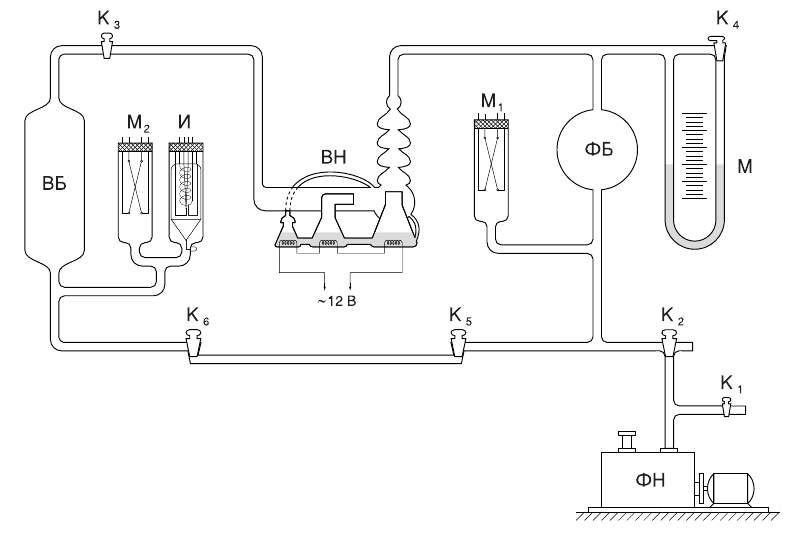
\includegraphics[scale=.6]{scheme.png}
	\end{center}
	\end{figure}
	
	Установка (\fref{fig:scheme}) изготовлена из стекла и состоит из форвакуумного баллона (ФБ), высоковакуумного диффузионного насоса (ВН), масляного (М) и ионизационного (И) манометров, термопарных манометров ($M_1$ и $M_2$), форвакуумного насоса (ФН) и соединительных кранов К. Кроме того, в состав установки входит вариатор (автотрансформатор с регулируемым выходным напряжением) или реостат и амперметр для регулирования тока нагревателя диффузионного насоса.
	
	\textit{Форвакуумный насос}. Устройство и принцип действия ротационного пластинчатого форвакуумного насоса схематически показаны на \fref{fig:scheme-fv}.
	
	\begin{figure}[h!]
	\caption{Схема действия форвакуумного насоса}
	\label{fig:scheme-fv}
	\begin{center}
	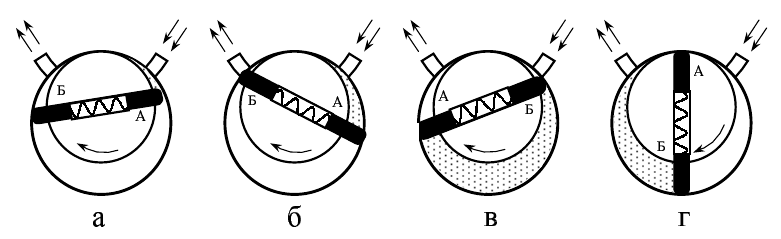
\includegraphics[scale=.6]{scheme1.png}
	\end{center}
	\end{figure}
	
	В цилиндрической полости массивного корпуса размещён эксцентрично ротор так, что он постоянно соприкасается своей верхней частью с корпусом. В диаметральный разрез ротора вставлены две пластины, которые с помощью пружины тщательно прижимаются к поверхности полости и разделяют объём между поверхностью и ротором на две части.
	
	В положениях <<а>> и <<б>> пластина <<А>> засасывает разреженный воздух из откачиваемого объёма, а пластина <<Б>> вытесняет ранее захваченный воздух в атмосферу. В положениях <<в>> и <<г>> они поменялись ролями.
	
	Насос подсоединяют к установке не сразу, а после того, как он откачает собственный объём.
	
	\textit{Диффузионный насос}. Откачивающее действие диффузионного насоса основано на внедрении (диффузии) молекул разреженного воздуха в струю паров масла. Попавшие в струю молекулы увлекаются ей и уже не возвращаются назад. Скорость откачки диффузионных насосов на два-три порядка превышает скорость откачки форвакуумного насоса.
	
	\begin{figure}[h!]
	\caption{Схема работы диффузионного насоса}
	\label{fig:scheme-dfn}
	\begin{center}
	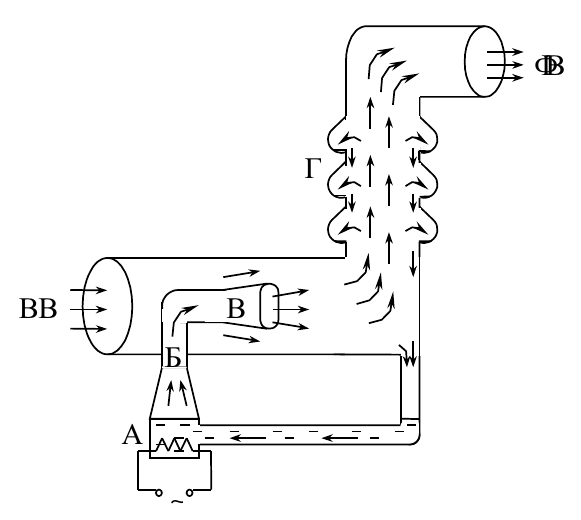
\includegraphics[scale=.6]{scheme2.png}
	\end{center}
	\end{figure}
	
	Устройство одной ступени масляного насоса показано на \fref{fig:scheme-dfn}. Масло в сосуде нагревается электрической печкой, пары поднимаются и вырываются из сопла, затем увлекают молекулы воздуха. Потом смесь попадает в вертикальную трубу. Масло осаждается на стенках трубы и маслосборников и стекает вниз, а оставшийся газ откачивается форвакуумным насосом через трубу. Диффузионный насос работает наиболее эффективно при давлении, когда длина свободного пробега приблизительно равна ширине зазора между соплом и стенкой вертикальной трубы.
	
	Давление насыщенных паров масла при рабочем давлении нанмого больше давления воздуха, за счёт чего создаётся плотная струя. Если включить насос при большом давлении воздуха, масло будет гореть, а не испаряться.
	
	В установке используется двухступенчатый насос, первое сопло вертикальное, второе --- горизонтальное. За второй ступенью ещё одна печь, которая разделяет масло на легко- и малолетучие фракции, подаваемые в первую и вторую ступень соотв. За счёт этого плотность струи второй ступени меньше и меньше давление насыщенных паров там, в объём поступает меньше масла и его можно откачать до более высокого вакуума, чем если бы ступень была одна.
	
	В диффузионном насосе масло надо нагревать постепенно, чтобы оно не загорелось и не стало кипеть слишком интенсивно.
	
	\textit{Масляный манометр} представляет собой просто U-образную трубку, наполненную вязким маслом (малое давление насыщенных паров). Нужно следить, чтобы из него не выбрасывалось масло.
	
	\textit{Термопарный манометр} состоит из платино-платинородиевой термопары, спаянной с никелевой нитью накала и заключённой в стеклянный баллон (\fref{fig:scheme-tman}). По нити накала НН пропускается ток постоянной величины, регулируемый потенциометром. Термопара присоединяется к милливольтметру, показания которого определяются её температурой и зависят от теплопроводности воздуха.
	
	\begin{figure}[h!]
	\caption{Схема термопарного манометра и градуировочная кривая}
	\label{fig:scheme-tman}
	\begin{center}
	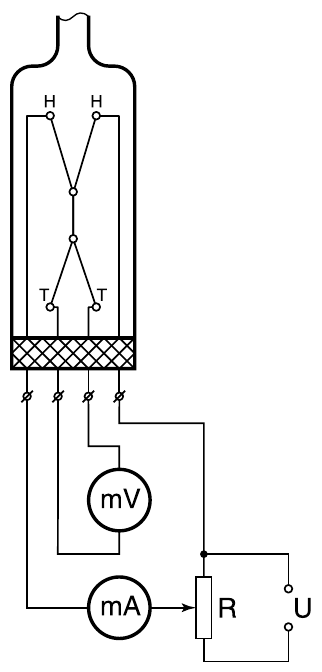
\includegraphics[scale=.6]{scheme3.png}
	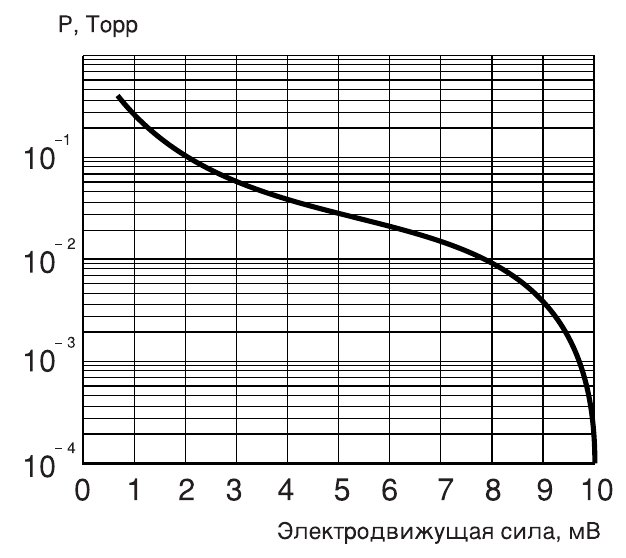
\includegraphics[scale=.6]{scheme4.png}
	\end{center}
	\end{figure}
	
	При давлениях более 1 торр теплопроводность почти не зависит от давления и прибор не работает. Градуировочная кривая термопары приведена на \fref{fig:scheme-tman}.
	
	\begin{figure}[h!]
	\caption{Ионизационный манометр}
	\label{fig:scheme-iman}
	\begin{center}
	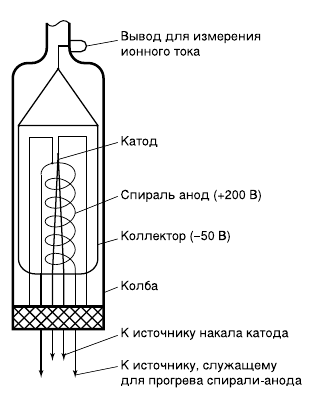
\includegraphics[scale=.6]{scheme5.png}
	\end{center}
	\end{figure}
	
	\textit{Ионизационный манометр} представляет собой трёхэлектронную лампу (\fref{fig:scheme-iman}). Электроны испускаются накалённым катодом и увлекаются электрическим полем к аноду, пролетают его, отталкиваются обратно полем коллектора и производят такое движение очень много раз, ионизируя молекулы газа, которые дают заметный вклад в ток.
	
	Вероятность ионизации зависит только от газа, поэтому ток служит мерой давления.
	
	Накалённый катод при больших давлениях перегорает, поэтому лампу нельзя включать, пока вакуум не будет достаточно откачан.
	
	При измерении нить накала сильно греется, и лампа может десорбировать поглощённый ранее газ, ухудшая вакуум. Поэтому её предварительно прогревают в течение 10--15 минут.
	
	\subsection*{Процесс откачки}
	
	Производительность насоса определяется скоростью откачки $W$ --- это объём газа, удаляемого из сосуда при данном давлении за единицу времени. Для форвакуумного насоса равна ёмкости воздухозаборной камеры, умноженной на число оборотов в секунду.
	
	Рассмотрим обычную схему откачки. Разделим установку на <<откачиваемый объём>> (рабочая часть) и <<насос>> (сам насос, а также трубки и краны, через которые происходит откачка. Обозначим $Q_\text{д}$ --- количество газа, десорбирующегося с поверхности, $Q_\text{и}$ --- количество газа, втекающего в объём извне (через течи), $W$ --- скорость откачки и $Q_\text{н}$ --- поток газа, поступающего из насоса назад. Будем измерять всё это в единицах $PV$ (масса с точностью до постоянного множителя). Основное уравнение:
	\begin{equation}
		\label{eq:otkach_main}
		-VdP=(PW-Q_\text{д}-Q_\text{и}-Q_\text{н})dt.
	\end{equation}
	
	При достижении предельного вакуума давление уже не меняется, тогда
	\begin{equation}
		\label{eq:otkach_bal_pred}
		PW=Q_\text{д}+Q_\text{и}+Q_\text{н}.
	\end{equation}
	
	Отсюда формула, выражающая скорость откачки через предельный вакуум:
	\begin{equation}
		\label{eq:otkach_sp_pred}
		W=\frac{\sum Q_i}{P_\text{пр}}.
	\end{equation}
	
	Обычно $Q_\text{и}$ постоянно, а остальные слабо зависят от времени, так что мы можем считать их постоянными. Считая постоянной и $W$, можно легко проинтегрировать \eqref{eq:otkach_main}:
	\begin{equation}
		\label{eq:otkach_sol}
		P-P_\text{пр}=(P_0-P_\text{пр}) \exp \left( -\frac{W}{V}t \right),
	\end{equation}
	где $P_0$ --- начальное давление. Обычно $P_0 \gg P_\text{пр}$, тогда
	\begin{equation}
		\label{eq:otkach_sol_approx}
		P=P_0 \exp \left( -\frac{W}{V}t \right).
	\end{equation}
	Постоянная времени $\tau=V/W$ является мерой эффективности системы откачки.
	
	Скорость откачки определяется пропускными способностями всех элементов <<насоса>>. При математическом описании для молекулярных течений возникают уравнения, похожие на уравнения Кирхгофа, и получается, что пропускные способности ведут себя как проводимости:
	\begin{equation}
		\label{eq:prop_abil}
		\frac{1}{W}=\frac{1}{W_\text{н}} + \sum_i \frac{1}{C_i},
	\end{equation}
	где $W_\text{н}$ --- пропускная способность насоса, $\{C_i\}$ --- пропускные способности элементов вакуумной системы.
	
	\subsection*{Течение газа через трубу}
	
	При давлениии, близком к атмосферному, течение газа определяется вязкостью. В высоком вакууме ситуация иная: столкновения со стенками начинают быть важнее, чем столкновения между молекулами.
	
	Для количества газа, протекающего через трубу в кнудсеновском режиме, справедлива формула
	\begin{equation}
		\label{eq:knudsen_stream}
		\frac{d(PV)}{dt}=\frac{4}{3}r^3 \sqrt{\frac{2\pi RT}{\mu}} \frac{P_2-P_1}{L}.
	\end{equation}
	
	Если пренебречь давлением у конца, обращённого к насосу, пропускная способность трубы
	\begin{equation}
		\label{eq:prop_abil_tube}
		C_\text{тр}=\left( \frac{dV}{dt} \right) _\text{тр} = \frac{4}{3} \frac{r^3}{L} \sqrt{\frac{2\pi RT}{\mu}}.
	\end{equation}
	Следовательно, трубы должны быть толстыми и короткими.
	
	Также необходимо учитывать пропускную способность отверстий. Для них поток выражается как
	\begin{equation}
		\label{eq:stream_otv}
		\upsilon=\frac{1}{4} Sn\bar{v}.
	\end{equation}
	
	Поскольку $P=nkT$, получим пропускную способность:
	\begin{equation}
		\label{eq:prop_abil_otv}
		C_\text{отв}=\frac{1}{4} S\bar{v}.
	\end{equation}
	
	Формулу \eqref{eq:prop_abil_otv} можно получить непосредственно из условия $$ \upsilon=C_\text{отв}n, $$ выражающего эквивалентность действия отверстия, открытого в высокий вакуум, и поршня, расширяющего объём со скоростью $C_\text{отв}$.
	
	Для диффузионного насоса можно считать, что каждая молекула, попавшая в струю масла, увлекается ей, поэтому скорость откачки почти равна пропускной способности отверстия кольцевого зазора, т.е. он качает как кольцевой зазор, открытый в пустоту.
	
	\section*{Ход работы}
	
	Параметры установки: $V_\text{кап}=(40\pm 2) \,\text{см}^3$, $L_\text{кап}=75$ мм, $d_\text{кап}=1{,}22$ мм, $P_0=99{,}6$ кПа, плотность масла $\rho=0{,}885\,\frac{\text{г}}{\text{см}^3}$.
	
	\subsection*{Определение объёма форвакуумной и высоковакуумной частей установки}
	
	\begin{enumerate}
		\item Открыли все краны, кроме $K_1$ и $K_2$.
		\item Впустили в установку атмосферный воздух.
		\item Закрыли $K_5$ и $K_6$, заперев в капилляре воздух.
		\item Откачали установку форвакуумным насосом до $10^{-2}$ торр.
		\item Отсоединили вакуумный насос от установки, выключили его, подали на него атмосферу.
		\item Закрыли $K_3$, отделив форвакуумную часть от высоковакуумной.
		\item Закрыли $K_4$, приведя в готовность масляный манометр.
		\item Открыли $K_5$.
		\item Измерили давление масляным манометром $\Delta h_\text{ФВ}=9$ см масл.ст.
		\item Открыли $K_3$.
		\item Измерили давление масляным манометром $\Delta h_\text{П}=6{,}5$ см масл.ст.
		\item Открыли $K_4$.
	\end{enumerate}
	
	\subsection*{Получение высокого вакуума и измерение скорости откачки}
	
	\begin{enumerate}
		\item Оставили установку без запертых частей, откачали форвакуумным насосом.
		\item Включили термопарные вакуумметры.
		\item Когда давление упало до $P_1=1{,}5\cdot 10^{-2}$ торр, закрыли $K_6$.
		\item Включили нагреватель диффузионного насоса и подождали 10 минут.
		\item Включили ионизационный манометр.
		\item Измерили предельное давление в системе $P_\text{пр}=1{,}2\cdot 10^{-4}$ торр.
		\item Измерили скорость откачки по улучшению: \label{exp_repeat}
		\begin{enumerate}
			\item отключили откачку краном $K_3$ и подождали, пока вакуум достаточно ухудшится.
			\item открыли $K_3$ и отмечали изменение показаний со временем.
		\end{enumerate}
		\item Измерили величину потока $Q_\text{н}$: перекрыли $K_3$ и записывали показания во времени. \label{exp_repeat_end}
		\item Повторили измерения по пп. \ref{exp_repeat}--\ref{exp_repeat_end} ещё дважды.
		\item Открыли $K_6$, дождались установления давления и записали его ($P_\text{уст}=1{,}9\cdot 10^{-4}$ торр).
		\item Выключили установку.
	\end{enumerate}
	
	\section*{Обработка результатов}
	
	По закону Бойля-Мариотта,
	\begin{equation}
		\label{eq:boile-mariotte}
		P_0 V_\text{кап}= \rho g \Delta h V,
	\end{equation}
	
	откуда
	\begin{equation}
		\label{eq:vol_working}
		V_\text{ФВ}= V_\text{кап} \frac{P_0}{\rho g \Delta h_\text{ФВ}}, V_\text{ВВ}= V_\text{кап} \frac{P_0}{\rho g} \left( \frac{1}{\Delta h_\text{ВВ}} - \frac{1}{\Delta h_\text{ФВ}} \right).
	\end{equation}
	
	Получаем, принимая погрешность определения разности уровней 0,5 см: $$ V_\text{ФВ}=(5{,}1\pm 0{,}4) \,\text{л}, $$  $$ V_\text{ВВ}=(2{,}0\pm 0{,}8) \,\text{л}. $$
	
	Затем для улучшения вакуума я построил график $\ln N(t)$ (\fref{graph_ul}), где $N$ -- показания ионизационного вольметра в соответствии с \eqref{eq:otkach_sol_approx}.
	
	\begin{figure}[!h]
		\caption{График зависимости показаний ионизационного вольтметра от времени (улучшение вакуума)}
		\label{graph_ul}
		\begin{center}
		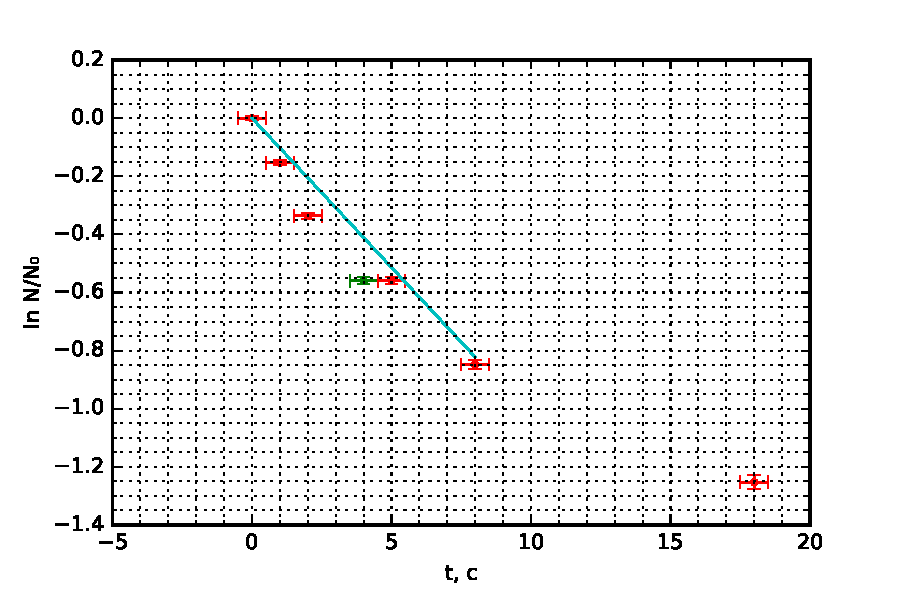
\includegraphics[scale=.8]{graph2.pdf}
		\end{center}
	\end{figure}
	
	Как видно, первые точки неплохо ложатся на прямую, но чем дальше, чем больше отклонение от неё. Причина, скорее всего, в том, что $P \sim P_\text{пр}$ в последних точках.
	
	Путём аппроксимации получено $$ \frac{1}{\tau}=(0{,}103\pm 0{,}005) \frac{1}{\text{с}}. $$ Тогда понятно, что $$ W=(0{,}20\pm 0{,}08) \frac{\text{л}}{\text{с}}. $$
	
	Также я построил аналогичный график для ухудшения вакуума (\fref{graph_uh}), он получился почти линейным в обычном масштабе.
	
	\begin{figure}[!h]
		\caption{График зависимости показаний ионизационного вольтметра от времени (ухудшение вакуума)}
		\label{graph_uh}
		\begin{center}
		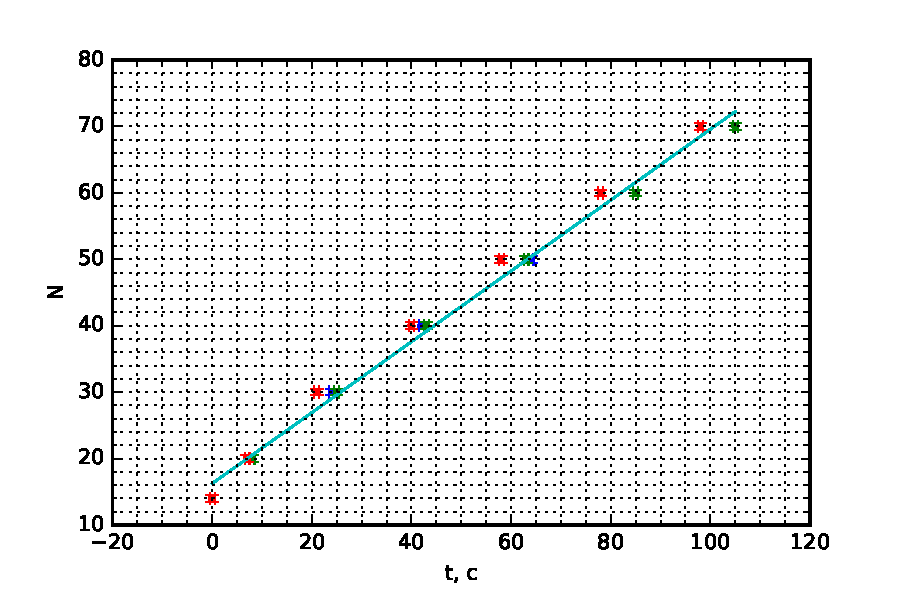
\includegraphics[scale=.8]{graph1.pdf}
		\end{center}
	\end{figure}
	
	Путём аппроксимации получено $$ \frac{dP}{dt}=(5{,}33\pm 0{,}11) \cdot 10^{-6} \frac{\text{торр}}{\text{с}}. $$
	
	Поскольку в этом случае $$ V_\text{ВВ} \frac{dP}{dt} = Q_\text{д}+Q_\text{и}, $$ получаем $$ Q_\text{н}=PW-V_\text{ВВ} \frac{dP}{dt}. $$
	
	Подсчёты дают результат $$ Q_\text{н} \approx 10^{-5} \frac{\text{торр} \cdot \text{л}}{\text{с}} $$
	
	Рассчитаем производительность насоса по различию $P_\text{уст}$ и $P_\text{пр}$. Запишем \eqref{eq:otkach_bal_pred} при открытом и закрытом капилляре: $$ P_\text{пр} W=Q_1, P_\text{уст} W = Q_1+\frac{d(PV)_\text{кап}}{dt}. $$ Вычтем одно из другого и подставим из \eqref{eq:knudsen_stream}:
	
	\begin{equation}
		\label{eq:otkach_by_pred_ust}
		W = \frac{4}{3} \sqrt{\frac{2\pi RT}{\mu}} \frac{r^3}{L} \frac{P_1-P_\text{уст}}{P_\text{уст} - P_\text{пр}}.
	\end{equation}
	
	Получаем $$ W=(0{,}66\pm 0{,}07) \frac{\text{л}}{\text{с}}. $$
	
	Вероятно, результаты не совпадают, потому что мы не достигли действительно предельного давления. Перед началом ухудшения вакуума мы наблюдали предельное давление раза в два ниже, но оно было утеряно.
	
\end{document}
